% #######################################
% ########### FILL THESE IN #############
% #######################################
\def\mytitle{LINE EQUATION USING INTERCEPT POINTS }
\def\mykeywords{}
\def\myauthor{DUDEKULA USENI}
\def\contact{r171099@rguktrkv.ac.in}
\def\mymodule{}
% #######################################
% #### YOU DON'T NEED TO TOUCH BELOW ####
% #######################################
\documentclass[10pt, a4paper]{article}
\usepackage[a4paper,outer=1.5cm,inner=1.5cm,top=1.75cm,bottom=1.5cm]{geometry}
\twocolumn
\usepackage{graphicx}
\graphicspath{{./images/}}
%colour our links, remove weird boxes
\usepackage[colorlinks,linkcolor={black},citecolor={blue!80!black},urlcolor={blue!80!black}]{hyperref}
%Stop indentation on new paragraphs
\usepackage[parfill]{parskip}
%% Arial-like font
\usepackage{lmodern}
\renewcommand*\familydefault{\sfdefault}
%Napier logo top right
\usepackage{watermark}
%Lorem Ipusm dolor please don't leave any in you final report ;)
\usepackage{circuitikz}
\usetikzlibrary{calc}
\usepackage{tikz}

\usetikzlibrary{shapes, arrows, chains, decorations.markings,intersections,calc}
\usepackage{lipsum}
\usepackage{xcolor}
\usepackage{listings}
%give us the Capital H that we all know and love
\usepackage{float}
%tone down the line spacing after section titles
\usepackage{titlesec}
%Cool maths printing
\usepackage{amsmath}
\usepackage{tabularx}
%PseudoCode
\usepackage{algorithm2e}
\newcommand{\myvec}[1]{\ensuremath{\begin{pmatrix}#1\end{pmatrix}}}
\let\vec\mathbf
\lstset{
frame=single, 
breaklines=true,
columns=fullflexible
}
\titlespacing{\subsection}{0pt}{\parskip}{-3pt}
\titlespacing{\subsubsection}{0pt}{\parskip}{-\parskip}
\titlespacing{\paragraph}{0pt}{\parskip}{\parskip}
\newcommand{\figuremacro}[5]{
    \begin{figure}[#1]
        \centering
        \includegraphics[width=#5\columnwidth]{#2}
        \caption[#3]{\textbf{#3}#4}
        \label{fig:#2}
    \end{figure}
}

\lstset{
frame=single, 
breaklines=true,
columns=fullflexible
}

\thiswatermark{\centering \put(-15,-100.0){
\includegraphics[scale=0.3]{logo}} }
\title{\mytitle}
  \author{\myauthor\hspace{1em}\\\contact\\FWC22098         IITH-Future Wireless Communications             Assignment-matrices\hspace{0.8em}\hspace{0.5em}\mymodule}
\date{}
\hypersetup{pdfauthor=\myauthor,pdftitle=\mytitle,pdfkeywords=\mykeywords}
\sloppy
% #######################################
% ########### START FROM HERE ###########
% #######################################
 
 \begin{document}
 \maketitle
     \tableofcontents 
    \begin{figure}
        \centering
        %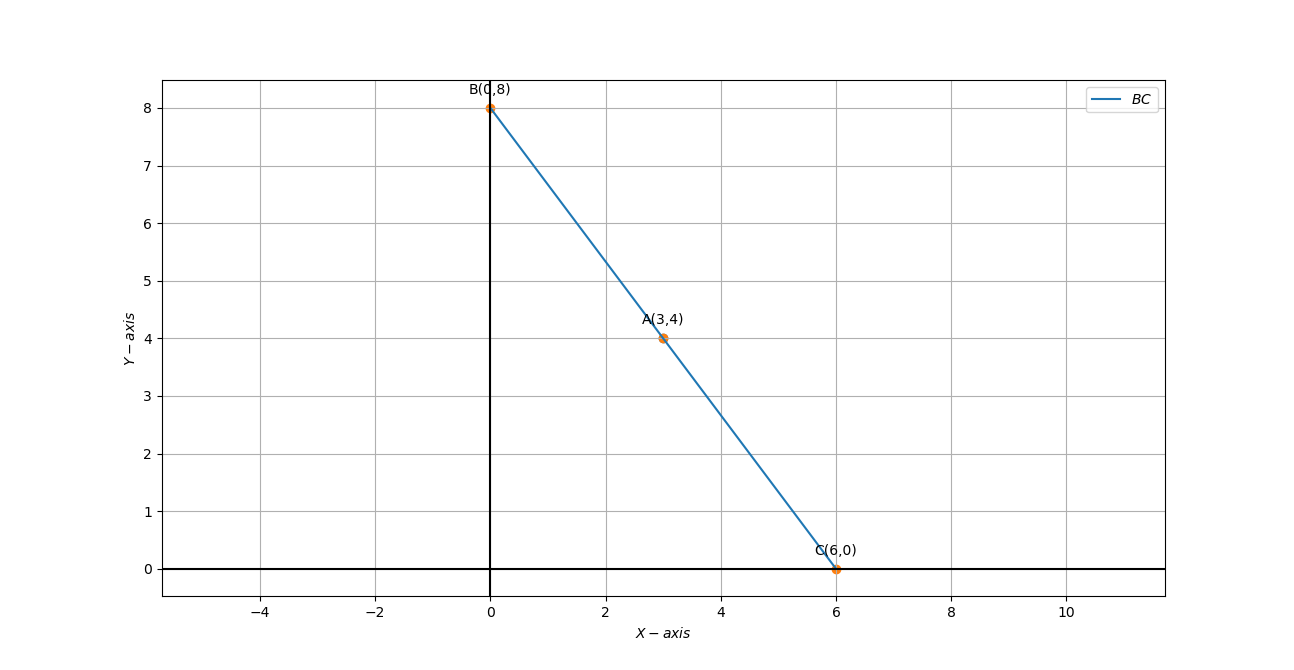
\includegraphics[scale=0.3]{line.png}
        %\caption{\textbf{The logic realised by the circuit shown in figure is}}
        \label{fig:my_label}
    \end{figure}
  \textbf{}{\mykeywords}
 \section{Problem}
 A straight line through the point A(3, 4) is such that its intercept between the axes is bisected at A. Its equation is :
      \section{Solution}
   \begin{center}
The input given 
\boldmath
$$A=\begin{pmatrix} 3\\ 4\ \end{pmatrix}$$
\end{center}
To prove \textbf{4x + 3y = 24}\\
The equation of a line is :
$$n^{\top}X=c$$
$$n^{\top}A=c$$
$$n^{\top}B=c$$
$$n^{\top}C=c$$
$$A = \frac{B+C}{2}$$
 \begin{center}
\begin{align}
B+C = 2A
\end{align}
\begin{align}
e_1^{\top}B=0
\end{align}
\begin{align}
e_2^{\top}C=0
\end{align}
Here $e_1$ and and $e_2$ are standard basis vectors 
$$e_1=\begin{pmatrix} 1\\ 0\ \end{pmatrix}  ,  e_2=\begin{pmatrix} 0\\ 1\ \end{pmatrix}$$
In equation(1) ,multiply on both sides by $e_1^{\top}$ 
$$e_1^{\top}(B+C)=2e_1^{\top}A$$
$$e_1^{\top}B+e_1^{\top}C=2e_1^{\top}A$$
$$e_1^{\top}C=2e_1^{\top}A$$
 \end{center}
$$\textbf{C}=\begin{pmatrix} 2e_1^{\top}A\\ 0\ \end{pmatrix}=\begin{pmatrix} 6\\ 0\ \end{pmatrix}$$
In equation(1) ,multiply on both sides by $e_2^{\top}$ 
$$e_2^{\top}(B+C)=2e_2^{\top}A$$
$$e_2^{\top}B+e_2^{\top}C=2e_2^{\top}A$$
$$e_2^{\top}B=2e_2^{\top}A$$

$$\textbf{B}=\begin{pmatrix} 0\\2e_2^{\top}A\ \end{pmatrix}=\begin{pmatrix} 0\\ 8\ \end{pmatrix}$$
$$\textbf{m}=\begin{pmatrix}C-A\end{pmatrix}$$
$$\textbf{m}=\begin{pmatrix} 3\\-4 \end{pmatrix}$$
here m is a direction vector\\
$$\textbf{n}=\myvec{0&-1 \\ 1&0}\textbf{m}$$\\
$$\textbf{n}=\begin{pmatrix} 4\\ 3\ \end{pmatrix}$$
Here n is a normal vector \\


The equation of a line with normal vector n and passing through the point A  formula :\\
$$n^{\top}(X-A)=0$$
$$\begin{pmatrix} \ 4 \   3\ \end{pmatrix}\begin{pmatrix}
\begin{pmatrix} x\\ y\ \end{pmatrix} - \begin{pmatrix} 3\\ 4\ \end{pmatrix}\end{pmatrix}=0$$
Hence prove equation of line :$$4x+3y=24$$ 
\unboldmath
\section{Construction}
 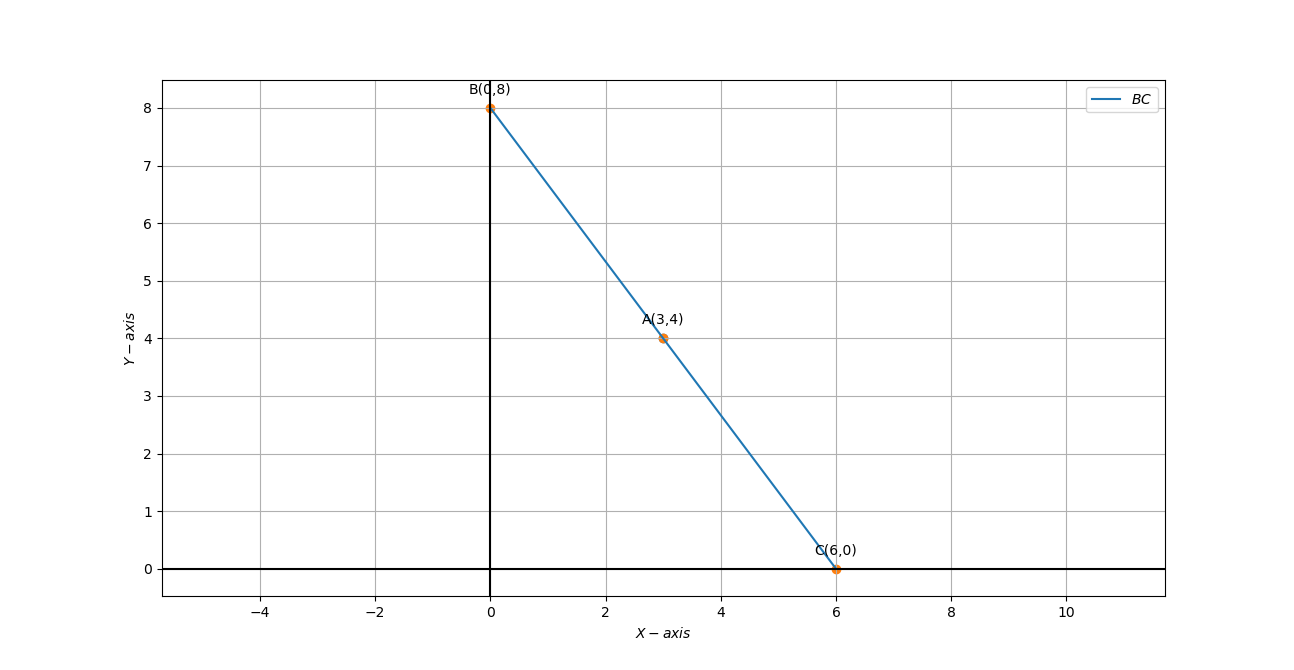
\includegraphics[scale=0.3]{line.png}
\section{Software}
 Download the following code
 \begin{lstlisting}
https://github.com/dudekulauseni123/FWC0982022
 \end{lstlisting}
\end{document}

   
 
